\documentclass[12pt,twoside]{book}

%Para listado de programas
\usepackage{listings}
\usepackage{color}

\definecolor{mygreen}{rgb}{0,0.5,0}
\definecolor{mygray}{rgb}{0.7,0.7,0.7}
\definecolor{mymauve}{rgb}{0.58,0,0.82}

\lstset{ %
	 backgroundcolor=\color{mygray},   % choose the background color; you must add \usepackage{color} or \usepackage{xcolor}
	 basicstyle=\footnotesize\ttfamily,        % the size of the fonts that are used for the code
	 breaklines=true,            % Zeilen werden Umgebrochen
	 keywordstyle=\color{red},
	 commentstyle=\itshape\color{mygreen},    % comment style
	 numbers=left,                    % where to put the line-numbers; possible values are (none, left, right)
	 numbersep=5pt                   % how far the line-numbers are from the code
}

%Paquete de Idioma
\usepackage[spanish]{babel}

%Codificación Alfabeto
\usepackage[utf8]{inputenc}

%Codificación de Fuente
\usepackage[T1]{fontenc}

%Índice
\usepackage{makeidx}

%Gráficos
\usepackage{graphicx}
\usepackage{float} 
%\usepackage{xcolor} 

%Matemática
\usepackage{amsmath}
\usepackage{amsfonts}
\usepackage{amssymb}
\usepackage{amstext} 

%Estilo de Página Numeración superior
%\pagestyle{headings}

%un estilo propio
\usepackage{fancyhdr}
\setlength{\headheight}{15pt}

\pagestyle{fancy}
\renewcommand{\chaptermark}[1]{ \markboth{\chaptername\ \thechapter: #1}{} }
\renewcommand{\sectionmark}[1]{ \markright{ Sección \thesection. #1}{} }

\fancyhf{}
\fancyhead[LE,RO]{\thepage}
\fancyhead[RE]{\textit{ \nouppercase{\leftmark}} }
\fancyhead[LO]{\textit{ \nouppercase{\rightmark}} }
\fancyfoot[CE]{\textit{\textcopyright 2016 Laboratorio de Sistemas Embebidos\\
	                    UPAEP} }
\fancyfoot[CO]{\textit{LSE001-2016 \\
		Elaboró: Dr. Casimiro Gómez González} }	            
\fancypagestyle{plain}{ %
	\fancyhf{} % remove everything
	\renewcommand{\headrulewidth}{0pt} % remove lines as well
	\renewcommand{\footrulewidth}{0pt}
}

%Hiperlinks \href{url}{text}
\usepackage[pdftex]{hyperref}

\usepackage{cite} % para contraer referencias

%Titulo
\title{LSE001-2016: Diplomado de Sistemas Embebidos para Automatización y Robótica}
\author{Dr. Casimiro Gómez González\\
	Facultad de Electrónica, UPAEP\\
               correo: casimiro.gomez@upaep.mx\\
               Tel: 2225 640517}
\date{Otoño de 2016}

\begin{document}

\maketitle

\chapter*{Prólogo}

El presente material ha sido elaborado en el laboratorio de sistemas embebidos UPAEP, y se ha desarrollado con la experiencia de estudiantes y profesores que han colaborado en dicho laboratorio. Hay material propio de clases y otro material generado a través de proyectos de vinculación y consultaría. Cualquier comentario o corrección favor de enviarlo por correo al autor.

\begin{flushright}
	
	El autor\\
	Casimiro Gómez González\\
	Doctor en Ingeniería Mecatrónica \\
	correo: casimiro.gomez@upaep.mx
\end{flushright}

\tableofcontents


\chapter{Conceptos Básicos de Sistemas Embebidos}

Los últimos diez años mas o menos, el mundo de la computación se ha movido desde las máquinas de escritorio grandes y estáticas a los dispositivos embebidos pequeños y móviles. Sistemas de software corriendo en redes de móviles, y los dispositivos embebidos deben tener propiedades que no siempre requieren los sistemas tradicionales:
\begin{itemize}
	\item Rendimiento cerca del óptimo
	\item Robustez
	\item Distribución
	\item Dinamismo
	\item Movilidad
\end{itemize}

Una de las diferencias en la ingeniería de software para sistemas embebidos es el conocimiento adicional que el ingeniero tiene de potencia eléctrica y electrónica; interfaces físicas de electrónica analógica y digital con la computadora; y diseño de software para sistemas embebidos y procesamiento digital de señales.

Cerca del 95\% de los sistemas de software son actualmente embebidos. Considera los dispositivos que tienes en casa de uso diario:

\begin{itemize}
	\item Teléfono Celular, iPOD, microondas
	\item receptor satelital de TV, receptor de TV de cable
	\item Unidad de control de automovil
	\item Reproductor de DVD
\end{itemize}

El desarrollo de software embebido usa los mismos modelos de desarrollo de software que las otras técnicas convencionales, incluyendo el modelo \textit{Waterfall}, el modelo en \textit{espiral} y el modelo \textit{Agile}.

\begin{figure}
	\centering
	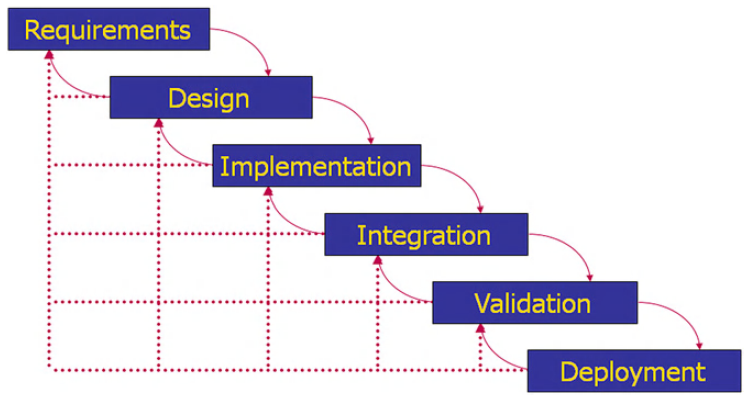
\includegraphics[width=0.9\linewidth]{waterfall.png}
	\caption{Modelo de desarrollo de software \textit{Waterfall}}
	\label{fig0001}
\end{figure}

\begin{figure}
	\centering
	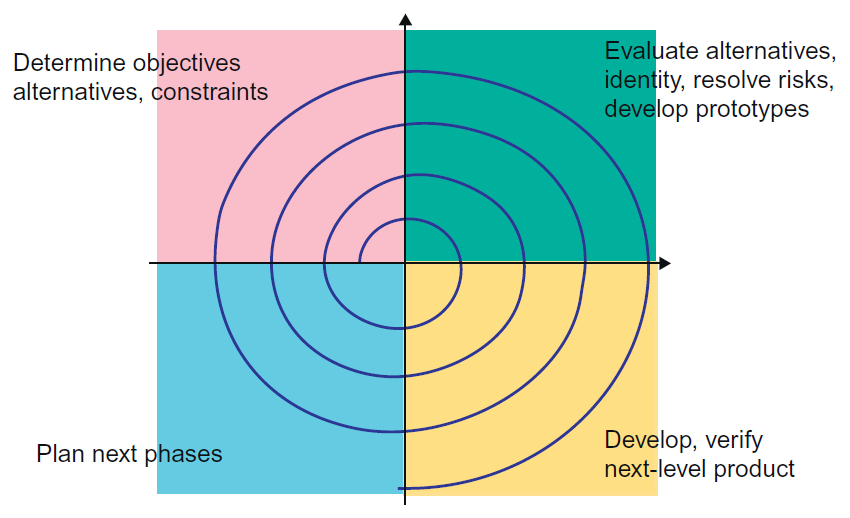
\includegraphics[width=0.9\linewidth]{espiral.png}
	\caption{Modelo de desarrollo de software \textit{Espiral}}
	\label{fig0002}
\end{figure}

\begin{figure}
	\centering
	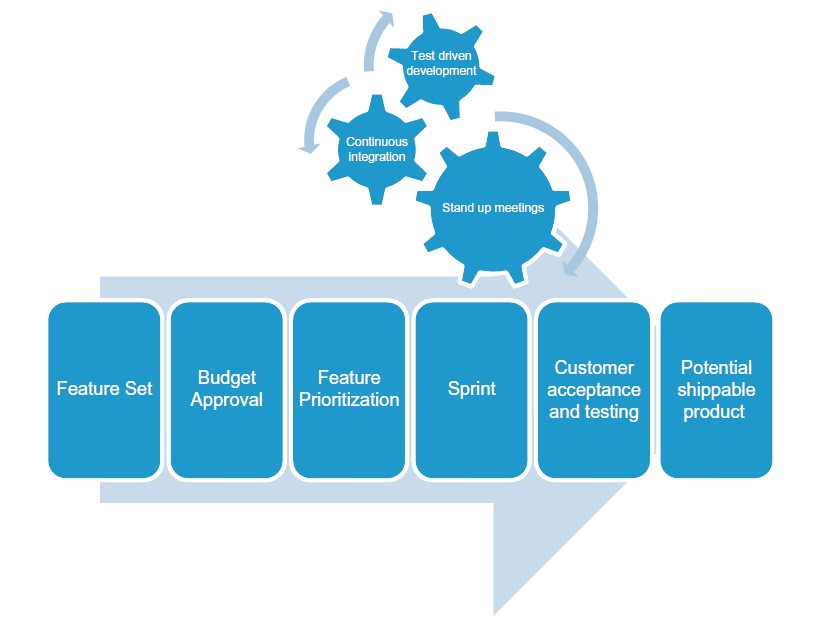
\includegraphics[width=0.9\linewidth]{agile.png}
	\caption{Modelo de desarrollo de software \textit{Agile}}
	\label{fig0003}
\end{figure}

La fases principales para el desarrollo de sistemas embebidos se pueden describir:
\begin{enumerate}
	\item \textbf{Definición del problema}: En esta fase se determina exactamente que quiere el cliente y el usuario. Esto incluye el desarrollo de un contrato con el cliente, dependiendo que tipo de producto esta siendo desarrollado. El objetivo de esta fase es especificar que producto de software se hará. Las dificultades incluyen: la solicitud del cliente por el producto incorrecto, el cliente no sabe sobre computación/software, lo cual limita la efectividad de esta fase, las especificaciones por lo regular son ambiguas, inconsistentes e incompletas.
	\item \textbf{Arquitectura/diseño}: La arquitectura se refiere a la selección de los elementos de arquitectónicos, sus interacciones, y las restricciones de aquellos elementos y sus interacciones necesarios para proporcionar un ambiente de trabajo con el cual satisfacer los requerimientos y servir como base para el diseño.  El diseño se refiere a la modularización y detalle de interfaz entre los elementos de diseño, sus algoritmos y procedimientos, y los tipos de datos necesarios para soportar la arquitectura y satisfacer los requerimientos. Durante la fase de arquitectura y diseño, el sistema es descompuesto en módulos de software con interfaces. Durante el diseño, el equipo de software desarrolla las especificaciones de los módulos (algoritmos y los tipos de datos),  manteniendo un récord de las decisiones de diseño y la trazabilidad, y especifica como los productos de software harán estas tareas. La dificultad principal durante esta fase incluye la falta de comunicación entre los diseñadores de módulos y terminan desarrollando un diseño que puede ser inconsistente, incompleto y ambiguo.
	\item \textbf{Implementación}: Durante esta fase el equipo de desarrollo implementa los módulos y componentes y verifica que cumplan las especificaciones. Los módulos se combinan de acuerdo con el diseño. Las implementaciones especifican como los productos del software hacen su trabajo. Algunas de las dificultades principales incluyen los errores de interacción entre los módulos y los errores de integración que pueden influenciar la calidad y la productividad.

	\item \textbf{Verificación y Validación(V\&V)}: Hay varias formas de V\&V. Una forma es el ``análisis''. El análisis puede ser en la forma de verificación estática, científica y formal y en revisiones informales. Las pruebas es una forma dinámica de V\&V. Esta forma de pruebas viene en la forma de una caja blanca (se tiene acceso al código) y de caja negra (no hay acceso al código). Las pruebas pueden ser estructurales o de comportamiento.Hay pruebas estándares para realizar dependiendo del producto a desarrollar.
	 
\end{enumerate}

Mas y mas desarrollo de software para sistemas embebidos se esta moviendo al desarrollo basado en componentes.Este tipo de desarrollo es aplicado generalmente para componentes de tamaño razonable y reutilización a través del sistema, que es una tendencia creciente en sistemas embebidos. Los desarrolladores aseguran que estos componentes son adaptables a contextos variantes y extienden la idea mas allá del código a otros artefactos desarrollados también. Esta técnica cambia la ecuación desde ``Integración, entonces Bajar al Hardware'' a ``Bajar al Hardware, entonces Implementar''.

\section{Definición formal de Sistemas Embebidos}

Se trata de un sistema de computación diseñado  para realizar una o algunas funciones dedicadas frecuentemente en un sistema de computación en tiempo real. Al contrario de lo que ocurre con los ordenadores de propósito general (como por ejemplo una computadora personal o PC) que están diseñados para cubrir un amplio rango de necesidades, los sistemas embebidos se diseñan para cubrir necesidades específicas.

\section{Historia}



\bibliographystyle{acm}
\bibliography{../bibliografia}

\end{document}